\documentclass{beamer} 
\usetheme{default} 
\usecolortheme{albatross}
\setbeamercovered{transparent}
%\useoutertheme{umbcfootline}  


\usepackage[spanish]{babel}
%\usepackage[latin1]{inputenc}
\usepackage[utf8x]{inputenc}
\usepackage{hyperref}
\usepackage{color}



%\usepackage{multicol}



\title{Entrada y Salida}

\author{Manuel J. Molino Milla \and Luis Molina Garzón}

\date{\today} %

\institute{IES Virgen del Carmen \and Departamento de Informática}




%\beamerdefaultoverlayspecification{<+->}

\begin{document}


\begin{frame}
  \titlepage
\end{frame}

\begin{frame}
    \frametitle{Logo}
\begin{figure}

\includegraphics[scale=1]{imagenes/logo.jpeg} 
\caption{Logo Java}
\end{figure}
\end{frame}

\begin{frame}
  \frametitle{Contenido}
  \tableofcontents[pausesections]
\end{frame}

\section{IO}
\begin{frame}
\frametitle{Introducción	}
\begin{description}[<+-|alert@+>]
\item[JDK 1.0] Introduce el paquete \emph{java.io}, I/O basada en stream
\item[JDK 1.4] Introduce el paquete \emph{java.nio}, I/O basada en buffer
\item[JDK 1.5] Introduce I/O de texto formateado con nuevas clases \emph{Scanner}, \emph{Formatter} o \emph{printf}
\item[JDK 1.7] mediante \emph{NIO.2} con I/O no bloqueante.
\end{description}
\pause
\end{frame}

\section{Flujos}
\begin{frame}[fragile]
\frametitle{Stream o flujos)}
\begin{itemize}[<+->]
\item Canal de comunicación en las operaciones I/O
\item Tenemos flujos de entrada y flujos de salida.
\item Nos da independencia de la procedencia de los datos (bits)
\begin{enumerate}
\item Entrada desde teclado.
\item Salida a monitor.
\item Lectura de un fichero.
\item Escritura en un fichero.
\item Evío y recepción de datos por red.
\end{enumerate}
\end{itemize}
\pause
\end{frame}

\begin{frame}
\frametitle{Flujos I/O}
\begin{figure}
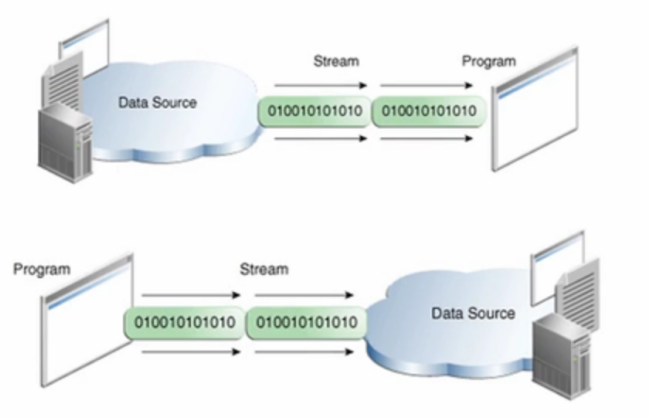
\includegraphics[scale=0.5]{imagenes/flujo.png}
\end{figure}
\end{frame}


\begin{frame}
\frametitle{Flujos I/O}
\begin{figure}
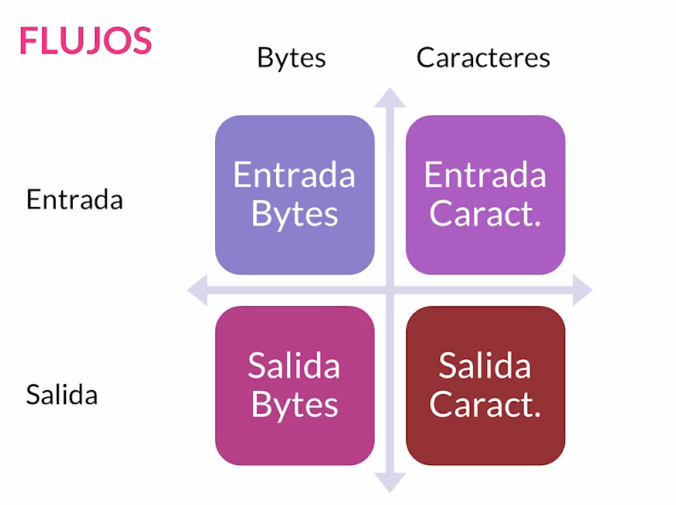
\includegraphics[scale=0.5]{imagenes/flujo1.png}
\end{figure}
\end{frame}

\begin{frame}[fragile]
\frametitle{Caracteres stream y byte stream}
Java almacena de forma interna los caracteres usando 16-bit  UCS-2. Pero la fuente de datos puede almacenar usando codificaciones diferentes como US-ASCII, ISO-8859-x, UTF-8, UTF-16, \dots\\
Java necesita diferenciar entre I/O basada en \alert{bytes}: procesamiento I/O raw bytes o binary data y en \alert{caracteres} usando dos bytes.\\
\begin{figure}
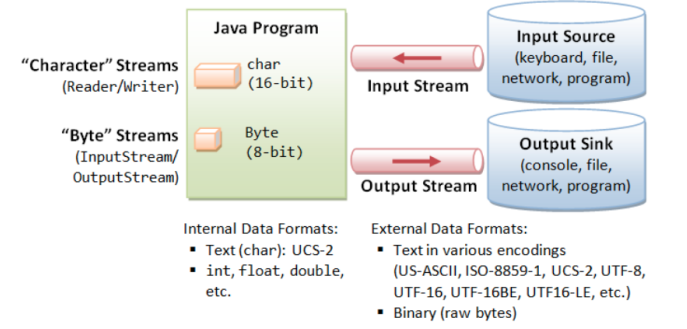
\includegraphics[scale=0.5]{imagenes/stream.png}
\end{figure}
\end{frame}




\section{Stream}
\begin{frame}[fragile]
\frametitle{Flujos de salida}
La forma de trabajar es la siguiente:
\begin{itemize}[<+->]
\item Abrir el flujo.
\item Mientras que haya datos vamos a escribir datos en el flujo.
\item Cerrar el flujo.
\end{itemize}
\end{frame}



\subsection{bytes stream}
\begin{frame}
\frametitle{InputStream y OutputStream}
\begin{figure}
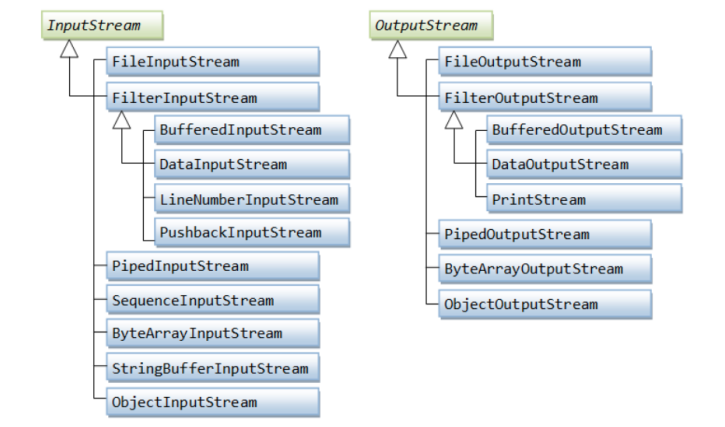
\includegraphics[scale=0.6]{imagenes/io.png}
\end{figure}
\end{frame}

\begin{frame}[fragile]
\frametitle{Flujos de salida de bytes}
\begin{description}[<+->]
\item[OutputStream] es la clase padre, abstracta, no se puede instanciar.
\item[FileOutputStream] permite escribir en un fichero byte a byte.
\item[BufferedOutputStream] permite escribir grupo de bytes, en vez de byte a byte
\item[ByteArrayOutputStream] permite escribir en memoria, obteniendo lo escrito en un \emph{array de bytes}
\pause
\end{description}
\end{frame}

\begin{frame}[fragile]
\frametitle{FileOutputStream}
Los usamos cuando estamos leyendos datos primitivos o String.
\pause
\begin{scriptsize}
\begin{verbatim}
  File file = new File("c:/newfile.txt");
  String content = "This is the text content";

  try (FileOutputStream fop = new FileOutputStream(file)) {

  // if file doesn't exists, then create it
    if (!file.exists()) {
      file.createNewFile();
    }

    // get the content in bytes
    byte[] contentInBytes = content.getBytes();

    fop.write(contentInBytes);
    fop.flush();

    System.out.println("Done");

  } catch (IOException e) {
    e.printStackTrace();
  }
\end{verbatim}
\end{scriptsize}
\end{frame}

\begin{frame}
\frametitle{BufferedOutputStream}
Volcamos el flujo de datos a otro
\begin{figure}
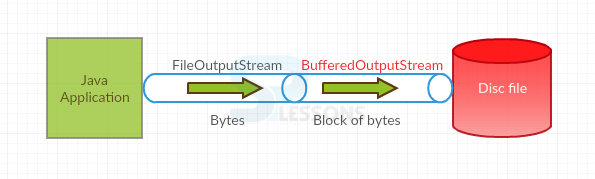
\includegraphics[scale=0.7]{imagenes/filebufferout.png}
\end{figure}
\end{frame}




\begin{frame}[fragile]
\frametitle{BufferedOutputStream}
%\begin{tiny}
\begin{verbatim}
try (BufferedOutputStream stream =
         new BufferedOutputStream(
           new FileOutputStream("textfile.txt"));){
  
    stream.write("Hello, World!".getBytes());
    stream.write(System.lineSeparator().getBytes());
    stream.write("I am writting into a file using " + 
                 "BufferedOutputStream".getBytes());
    stream.write(System.lineSeparator().getBytes());
    stream.close();
  } catch (IOException ex) {
    ex.printStackTrace();
  }
\end{verbatim}
%\end{tiny}
\end{frame}

\begin{frame}[fragile]
\frametitle{Data-Streams formateados: DataOutputStream}
Los usamos cuando estamos escribiendo datos primitivos o String.
\pause
\begin{verbatim}
DataOutputStream out = new DataOutputStream(
                        new BufferedOutputStream(
                         new FileOutputStream("out.dat")));
\end{verbatim}
\end{frame}

\begin{frame}[fragile]
\frametitle{Métodos de Data-Streams}
\begin{tiny}
\begin{verbatim}
public final void writeInt(int i) throws IOExcpetion;   // escribe 4 bytes
public final void writeFloat(float f) throws IOExcpetion;
public final void writeDoube(double d) throws IOExcpetion; // 
public final void writeByte(int b) throws IOExcpetion;     // 
public final void writeShort(int s) throws IOExcpetion;    // 
public final void writeLong(long l) throws IOExcpetion;
public final void writeBoolean(boolean b) throws IOExcpetion;
public final void writeChar(int i) throws IOExcpetion;
 
// String
public final void writeBytes(String str) throws IOExcpetion;  
public final void writeChars(String str) throws IOExcpetion;
     // Escribe String como UCS-2 16-bit char, Big-endian 
public final void writeUTF(String str) throws IOException;   
     // Escribe String como UTF, 2 bytes indican longitud de UTF bytes 

public final void write(byte[] b, int off, int len) throws IOException
public final void write(byte[] b) throws IOException
public final void write(int b) throws IOException 
\end{verbatim}
\end{tiny}
\end{frame}

\begin{frame}[fragile]
\frametitle{DataOutputStream}
%\begin{tiny}
\begin{verbatim}
double[] precios={1350, 400, 890, 6200, 8730};
  int[] unidades={5, 7, 12, 8, 30};
  String[] descripciones={"paquetes de papel", "lápices", 
                       "bolígrafos", "carteras", "mesas"};

  DataOutputStream salida=new DataOutputStream(
     new FileOutputStream("pedido.txt"));
  for (int i=0; i<precios.length; i ++) {
      salida.writeChars(descripciones[i]);
      salida.writeChar('\n');
      salida.writeInt(unidades[i]);
      salida.writeChar('\t');
      salida.writeDouble(precios[i]);
  }
  salida.close();
\end{verbatim}
%\end{tiny}
\end{frame}

\begin{frame}
\frametitle{Flujos de salida de caracteres}
\begin{figure}
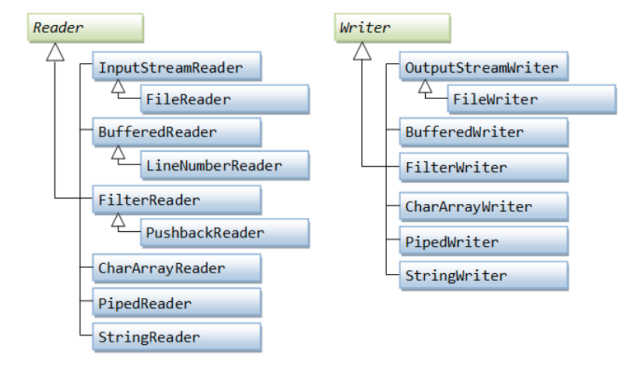
\includegraphics[scale=0.5]{imagenes/rw.png}
\end{figure}
\end{frame}


\begin{frame}[fragile]
\frametitle{Flujos de salida de caracteres}
\begin{description}[<+->]
\item[Writer] es la clase padre, abstracta, no se puede instanciar.
\item[FileWriter] permite escribir en un fichero caracter a caracter.
\item[BufferedWriter] permite escribir grupo de caracteres, en vez de caracter a caracter
\item[StringWriter] permite escribir en memoria, obteniendo lo escrito en un \emph{String}
\item[OutputStreamWriter] permite convertir un \emph{OutputStream} en un \emph{Writer}
\item[PrintWriter] flujo que permite escribir datos básicos de Java.
\end{description}
\pause
\end{frame}

\begin{frame}[fragile]
\frametitle{FileWriter}
%\begin{tiny}
\begin{verbatim}
FileWriter fw = null;
String intro = "En un lugar de La Mancha," +
                " de cuyo nombre no quiero acordarme";

try {
  fw = new FileWriter("introquijote.txt");
  for(char c : intro.toCharArray())
    fw.write(c);
} catch (IOException e) {
  e.printStackTrace();
} finally {
    if (fw != null)
       try {
             fw.close();
       } catch (IOException e) {
             e.printStackTrace();
       }
}
\end{verbatim}
%\end{tiny}
\end{frame}


\begin{frame}[fragile]
\frametitle{BufferedWriter}
\begin{scriptsize}

\begin{verbatim}
BufferedWriter bw = null;
List<String> quijote = Arrays.asList(new String[]
       { "En un lugar de la Mancha,", "de cuyo nombre no quiero acordarme,",
         "no ha mucho tiempo que vivía un hidalgo",
         "de los de lanza en astillero,", 
         "adarga antigua, rocín flaco y galgo corredor." });

try {
      bw = new BufferedWriter(new FileWriter("quijote.txt"));
      for (String s : quijote) {
            bw.write(s);
            bw.newLine();
      }
} catch (IOException e) {
      e.printStackTrace();
} finally {
      if (bw != null)
      try {
          bw.close();
      } catch (IOException e) {
          e.printStackTrace();
      }
}
\end{verbatim}
\end{scriptsize}
\end{frame}

\begin{frame}[fragile]
\frametitle{PrintStream \& PrintWriter}
\begin{itemize}[<+->]
\item La clase \emph{PrintStream} y \emph{PrintWriter} se usa para escribir texto formateado bajo \emph{OutputStream}
\item Tenemos métodos como \emph{print}, \emph{printf} o \emph{format}
\end{itemize}
\pause
\begin{small}
\begin{verbatim}
import java.io.*;
public class Print{
        public static void main(String[] arg) throws Exception{
              PrintStream output = new PrintStream(
                 new FileOutputStream(new File("hola.txt")));
              output.println(true);
              output.println((int) 123);
              output.println((float) 123.456);
              output.printf("%.2f %n", 12.3698);
              output.close();
        }
}
\end{verbatim}
\end{small}
\end{frame}

\begin{frame}
\frametitle{PrintStream \& PrintWriter}
\begin{figure}
\includegraphics[scale=0.8]{imagenes/PW.png}
\end{figure}
\end{frame}

\begin{frame}[fragile]
\frametitle{Problemas de codificación}
Lectura de un fichero con codificación iso-8859-1
\begin{verbatim}
try (BufferedReader in = new BufferedReader(
     new InputStreamReader(
         new FileInputStream("prueba2.txt"), "iso-8859-1"));) {
            String linea;
            while ((linea = in.readLine()) != null)
                  System.out.println(linea);
} catch (IOException e) {
         e.printStackTrace();
}
\end{verbatim}
Para una escritura
\begin{verbatim}
BufferedWriter out = new BufferedWriter(
  new OutputStreamWriter(
     new FileOutputStream("prueba3.txt"), "iso-8859-1"))
\end{verbatim}
\end{frame}


\begin{frame}
\frametitle{Flujos de entrada}
\begin{figure}
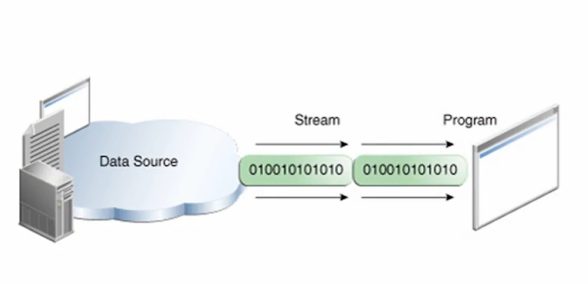
\includegraphics[scale=0.6]{imagenes/flujoEntrada.png}
\end{figure}
\end{frame}

\begin{frame}
\frametitle{Flujos de entrada}
\begin{figure}
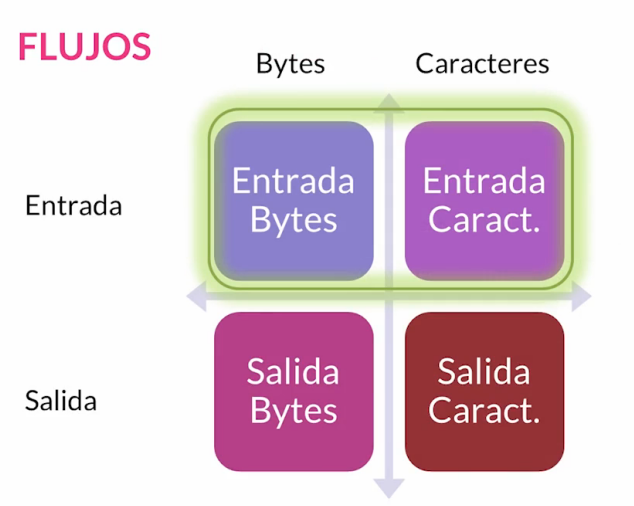
\includegraphics[scale=0.5]{imagenes/flujoEntrada1.png}
\end{figure}
\end{frame}


\begin{frame}
\frametitle{Flujos de entrada}
\begin{figure}
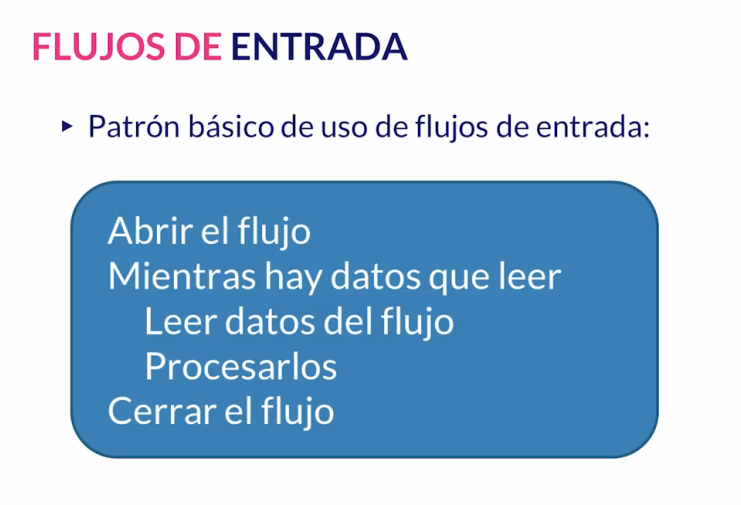
\includegraphics[scale=0.5]{imagenes/flujoEntrada2.png}
\end{figure}
\end{frame}


\begin{frame}
\frametitle{Flujos de entrada}
\begin{figure}
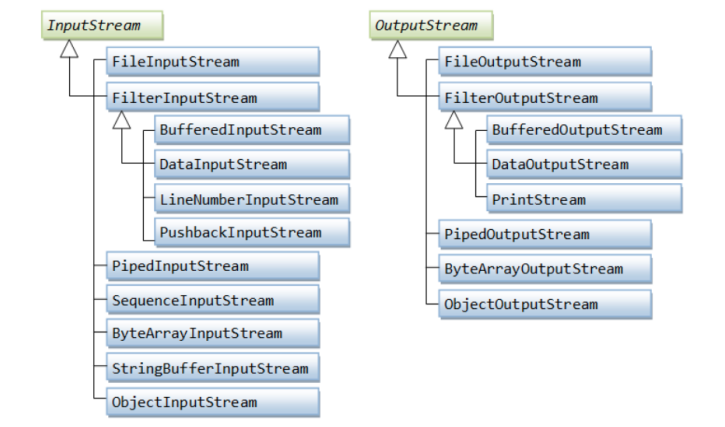
\includegraphics[scale=0.5]{imagenes/io.png}
\end{figure}
\end{frame}


\begin{frame}[fragile]
\frametitle{Flujos de entrada de bytes}
\begin{description}[<+->]
\item[InputStream] es la clase padre, abstracta, no se puede instanciar.
\item[FileInputStream] permite leer del fichero byte a byte.
\item[BufferedInputStream] permite leer grupo de bytes, en vez de byte a byte.
\item[ByteArrayInputStream] flujo que permite leer de memoria un array de bytes.
\end{description}
\pause
\end{frame}

\begin{frame}
\frametitle{Flujos de entrada de caracteres}
\begin{figure}
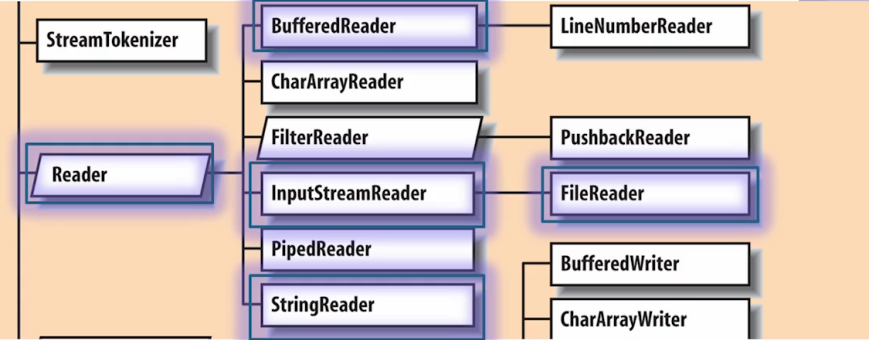
\includegraphics[scale=0.5]{imagenes/flujoEntradaCaracter.png}
\end{figure}
\end{frame}

\begin{frame}[fragile]
\frametitle{Flujos de entrada de caracteres}
\begin{description}[<+->]
\item[Reader] es la clase padre, abstracta, no se puede instanciar.
\item[FileReader] permite leer del fichero caracter a caracter.
\item[BufferedReader] permite leer grupo de caracteres, en vez de caracter a caracter.
\item[StringReader] flujo que permite leer de memoria un array de caracteres.
\item[InputStreamReader] Permite transformar un \emph{InputStrema} en un \emph{Reader}.

\end{description}
\pause
\end{frame}

\begin{frame}[fragile]
\frametitle{Ejemplo sin buffer}
%\begin{tiny}
\begin{verbatim}
import java.io.*;
public class FicherosBinariosApp {
  public static void main(String[] args) {
 
    try(FileInputStream fis=new FileInputStream(
          "D:\\fichero_bin.ddr")){
        int valor=fis.read();
        while(valor!=-1){
           System.out.print((char)valor);
           valor=fis.read();
        }
 
     }catch(IOException e){
           //....... 
     }
   }
}
\end{verbatim}
%\end{tiny}
\end{frame}

\begin{frame}[fragile]
\frametitle{Ejemplo con buffer}
\begin{tiny}

\begin{verbatim}
      InputStream inStream = null;
      BufferedInputStream bis = null;
      
      try {
         // open input stream test.txt for reading purpose.
         inStream = new FileInputStream("c:/test.txt");

         // input stream is converted to buffered input stream
         bis = new BufferedInputStream(inStream);			

         // read until a single byte is available
         while(bis.available()>0) {
         
            // read the byte and convert the integer to character
            char c = (char)bis.read();

            // print the characters
            System.out.println("Char: "+c);;
         }
      } catch(Exception e) {
         // if any I/O error occurs
         e.printStackTrace();
      } finally {		
         // releases any system resources associated with the stream
         if(inStream!=null)
            inStream.close();
         if(bis!=null)
            bis.close();
      }
\end{verbatim}
\end{tiny}
\end{frame}


\begin{frame}[fragile]
\frametitle{Entrada flujo char}
\begin{tiny}
\begin{verbatim}
import java.io.*;
// Write a text message to an output file, then read it back.
// FileReader/FileWriter uses the default charset for file encoding.
public class BufferedFileReaderWriterJDK7 {
   public static void main(String[] args) {
      String strFilename = "out.txt";
      String message = "Hello, world!\nHello, world again!\n";  

      // Print the default charset
      System.out.println(java.nio.charset.Charset.defaultCharset());
 
      try (BufferedWriter out = new BufferedWriter(new FileWriter(strFilename))) {
         out.write(message);
         out.flush();
      } catch (IOException ex) {
         ex.printStackTrace();
      }
 
      try (BufferedReader in = new BufferedReader(new FileReader(strFilename))) {
         String inLine;
         while ((inLine = in.readLine()) != null) {  // exclude newline
            System.out.println(inLine);
         }
      } catch (IOException ex) {
         ex.printStackTrace();
      }
   }
}
\end{verbatim}
\end{tiny}
\end{frame}


\begin{frame}[fragile]
\frametitle{Serialización y Object Streams}
\begin{itemize}[<+->]
\item \emph{ObjectInputStream y ObjectOutputStream} nos permite leer y escribir objetos.
\item Esos objetos pueden ser \emph{ArrayList, Date o cualquier objeto que creemos}
\item La \emph{serialización} es el proceso consistente en convertir un objeto en un flujo de bytes (\emph{stream}).
\item La serialización de un objeto es necesaria bien cuando guardamos el estado del objeto en disco o lo enviámos a través de la red.
\item Para que un objeto se pueda serializar debe implementar una de las dos siguientes interfaces: \emph{java.io.Serializable} o \emph{java.io.Externalizable}
\end{itemize}
\pause
\begin{verbatim}
public final Object readObject() throws IOException, 
   ClassNotFoundException;
public final void writeObject(Object obj) 
   throws IOException;
\end{verbatim}
\end{frame}


\section{Random Access Files}
\begin{frame}[fragile]
\frametitle{Acceso no secuencial de ficheros}
\begin{itemize}[<+->]
\item Los \emph{stream} que hemos visto o son de escritura o de lectura.
\item También existen \emph{stream} de acceso sencuencial.
\item Valen tanto para la lectura como para la escritura.
\item Lo que nos permiten modificar así como insertar nuevos datos.
\item La clase a usar el la clase \emph{RandomAccessFile}
\item \emph{RandomAccessFile} es como un gran array de bytes. Con un puntero localizado en la posición 0 al abrir el \emph{stream}
\item Dicho puntero avanza con la lectura de un número de bytes.
\end{itemize}
\pause
\begin{figure}
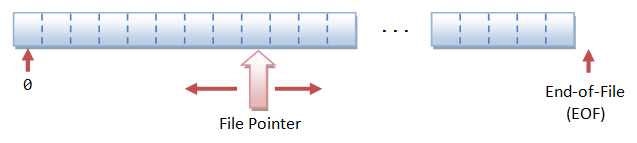
\includegraphics[scale=0.6]{imagenes/random.png}
\end{figure}
\end{frame}

\begin{frame}[fragile]
\frametitle{RandomAccessFile}
\begin{tiny}
\begin{block}{Constructores}
\begin{verbatim}
RandomAccessFile f1 = new RandomAccessFile("filename", "r");
RandomAccessFile f2 = new RandomAccessFile("filename", "rw");
\end{verbatim}
\end{block}
\pause
\begin{block}{Métodos sobre el puntero}
\begin{verbatim}
public void seek(long pos) throws IOException;
// posiciona el puntero en nueva posición.
public int skipBytes(int numBytes) throws IOException;
// Desplaza el puntero una serie de  bytes.
public long getFilePointer() throws IOException;
// Obtiene la posicion del puntero
public long length() throws IOException;
// Devuelve el tamaño del fichero.
\end{verbatim}
\end{block}
\pause
\begin{block}{Métodos de lectura/escritura}
\begin{verbatim}
public int readInt() throws IOException;
public double readDouble() throws IOException;
public void writeInt(int i) throws IOException;
public void writeDouble(double d) throws IOException;
\end{verbatim}
\end{block}
\end{tiny}
\end{frame}

\begin{frame}[fragile]
\frametitle{Ejemplo}
\begin{tiny}
\begin{verbatim}
import java.io.*;
public class TestRandomAccessFile{
  public static void main (String[]args) throws IOException  {
// Create a random-access file
    RandomAccessFile inout = new RandomAccessFile ("inout.dat", "rw");
// Clear the file to destroy the old contents, if any
      inout.setLength (0);
// Write new integers to the file
    for (int i = 0; i < 200; i++)
        inout.writeInt (i);
// Display the current length of the file
      System.out.println ("Current file length is " + inout.length ());
// Retrieve the first number
      inout.seek (0);           // Move the file pointer to the beginning
      System.out.println ("The first number is " + inout.readInt ());
// Retrieve the second number
      inout.seek (1 * 4);       // Move the file pointer to the second number
      System.out.println ("The second number is " + inout.readInt ());
// Retrieve the tenth number
      inout.seek (9 * 4);       // Move the file pointer to the tenth number
      System.out.println ("The tenth number is " + inout.readInt ());
// Modify the eleventh number
      inout.writeInt (555);
// Append a new number
      inout.seek (inout.length ());     // Move the file pointer to the end
      inout.writeInt (999);
// Display the new length
      System.out.println ("The new length is " + inout.length ());
// Retrieve the new eleventh number
      inout.seek (10 * 4);      // Move the file pointer to the next number
      System.out.println ("The eleventh number is " + inout.readInt ());
      inout.close ();
  }
}
\end{verbatim}
\end{tiny}
\end{frame}


\begin{frame}[fragile]
\frametitle{Ejemplos de ObjectInputStream \& ObjectOutputStream}
\begin{verbatim}
ObjectOutputStream out =
   new ObjectOutputStream(
      new BufferedOutputStream(
         new FileOutputStream("object.ser")));
out.writeObject("The current Date and Time is "); 
out.writeObject(new Date());                      
out.flush();
out.close();
\end{verbatim}
\pause
\begin{verbatim}
ObjectInputStream in = 
   new ObjectInputStream(
      new BufferedInputStream(
         new FileInputStream("object.ser")));
String str = (String)in.readObject();
Date d = (Date)in.readObject(new Date());  
in.close();
\end{verbatim}
\end{frame}

\begin{frame}[fragile]
\frametitle{Seriealización}
\begin{itemize}[<+->]
\item Los datos primitivos y array, por defecto son serializables.
\item Los campos estáticos no son serializables.
\item Si queremos que ciertos campos no sean serializables usamos el modificador \emph{trasient}
\item A veces aparece el mensaje \emph{Warning Message "The serialization class does not declare a static final serialVersionUID field of type long" (Advanced)}
\item Debido que algunas clases ya implementan la interfaz \emph{Serializable}
\item Para evitar este mensaje podemos hacer:
\begin{enumerate}
\item Ignorar el mensaje.
\item Añadir un id: \emph{private static final long serialVersionUID = 1L;}
\item Usar la notación $@$SuppressWarnings: \emph{@SuppressWarnings(''serial'')
public class MyFrame extends JFrame \{ ...... \}}
\end{enumerate}
\end{itemize}
\end{frame}




\begin{frame}[fragile]
\frametitle{Clase File}
\begin{itemize}[<+->]
\item Clase fundamental hasta java 6
\item A partir de NIO.2 pasa a un segundo plano.
\item Nos permite manejar ficheros y escritorios.
\end{itemize}
\pause
\begin{small}
\begin{verbatim}
File f = new File("file.txt"); 
  System.out.println("File name :"+f.getName()); 
  System.out.println("Path: "+f.getPath()); 
  System.out.println("Absolute path:" +f.getAbsolutePath()); 
  System.out.println("Parent:"+f.getParent()); 
  System.out.println("Exists :"+f.exists()); 
  if(f.exists()) 
    { 
      System.out.println("Is writeable:"+f.canWrite()); 
      System.out.println("Is readable"+f.canRead()); 
      System.out.println("Is a directory:"+f.isDirectory()); 
      System.out.println("File Size in bytes "+f.length()); 
    } 
\end{verbatim}
\end{small}
\end{frame}

\begin{frame}[fragile]
\frametitle{Creación de ficheros}
\begin{footnotesize}

\begin{verbatim}
try{
  //create a temp file
  File temp = File.createTempFile("temp-file-name", ".tmp"); 
  System.out.println("Temp file : " + temp.getAbsolutePath());
}catch(IOException e){
  e.printStackTrace();
}
\end{verbatim}
\pause
\begin{verbatim}
File file = new File("c://temp//testFile1.txt");
//Create the file
if (file.createNewFile())
{
   System.out.println("File is created!");
} else {
   System.out.println("File already exists.");
}
//Write Content
FileWriter writer = new FileWriter(file);
writer.write("Test data");
writer.close();
\end{verbatim}
\end{footnotesize}
\end{frame}



\begin{frame}
\frametitle{Path en Java}
\begin{figure}
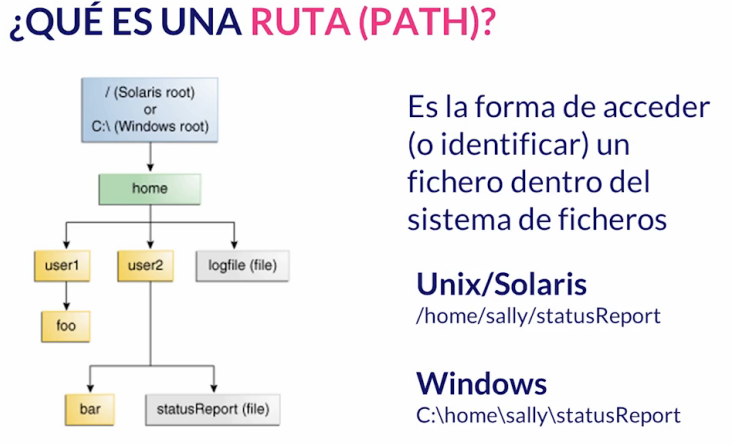
\includegraphics[scale=0.5]{imagenes/path.png}
\end{figure}
\end{frame}


\begin{frame}
\frametitle{Tipos de path}
\begin{block}{ruta absoluta}
\emph{/home/user/workspace/Proyecto\\
C:$\backslash$user$\backslash$workspace$\backslash$Proyecto}
\end{block}
\pause
\begin{block}{ruta relativa}
\emph{workspace/Proyecto}
\end{block}
\end{frame}


\begin{frame}[fragile]
\frametitle{Interfaz Path}
\begin{itemize}[<+->]
\item Introducida en Java 7
\item Representa una ruta en el sistema de ficheros.
\item Utiliza el nombre del fichero y los directorios padres.
\item Se suele usar la clase \emph{Paths} y sus métodos estáticos.
\end{itemize}
\pause
\end{frame}

\begin{frame}[fragile]
\frametitle{Ejemplo de Path}
\begin{small}
\begin{verbatim}
Path path = Paths.get(System.getProperty("user.home"),
                      "documentos", "java", "temario.txt");

System.out.format("toString: %s%n", path.toString());
System.out.format("getFileName: %s%n", path.getFileName());
System.out.format("getName(0): %s%n", path.getName(0));
System.out.format("getNameCount: %d%n", path.getNameCount());
System.out.format("subpath(0,2): %s%n", path.subpath(0,2));
System.out.format("getParent: %s%n", path.getParent());
System.out.format("getRoot: %s%n", path.getRoot());
\end{verbatim}
\end{small}
\end{frame}



\begin{frame}[fragile]
\frametitle{Clase Files}
\begin{itemize}[<+->]
\item Introduce muchos métodos estáticos
\item Algunos como comprobación de la existencia del fichero, conocer atributos de lectura, escritura, \dots
\item Métodos para copiar, borrar, mover, \dots
\item Métodos para trabajar con directorios.
\item Creación de ficheros regulares y temporales.
\item Flujos sin \emph{buffered} \emph{newInputStream} y \emph{newOutputStream}
\item \emph{buffer} con \emph{newBufferedReader} y \emph{newBufferedWriter}
\end{itemize}
\pause
\end{frame}

\begin{frame}[fragile]
\frametitle{Ejemplo I}
\begin{verbatim}
Path p = Paths.get("file.txt");
  if (Files.notExists(p)) {
    System.out.println("La ruta no existe");
       try {
           Files.createFile(p);
       } catch (IOException e) {
           e.printStackTrace();
       }
  }

  if (Files.exists(p))
      System.out.println("La ruta sí existe");

  if (Files.notExists(p))
      System.out.println("La ruta no existe");

     ........................
\end{verbatim}
\end{frame}

\begin{frame}[fragile]
\frametitle{Ejemplo II}
\begin{small}
\begin{verbatim}
//Creamos una ruta para crear un fichero
Path p = Paths.get("files", "fichero.txt");

//Creamos un fichero, y abrimos el flujo de texto para escribir
BufferedWriter bw = Files.newBufferedWriter(p);
bw.write("escritura de una cadena usando buffered");
bw.close();

//Copiamos el fichero
Path copia = Paths.get("files", "fichero_copiado.txt");
Files.copy(p, copia, StandardCopyOption.REPLACE_EXISTING);

//Lo movemos fuera del directorio
Files.move(copia, Paths.get("files", "copiado.txt"),
               StandardCopyOption.REPLACE_EXISTING);

//Lo eliminamos
Files.deleteIfExists(Paths.get("files", "copiado.txt"));

     ........................
\end{verbatim}
\end{small}
\end{frame}


\begin{frame}[fragile]
\frametitle{Ejemplo III}
\begin{footnotesize}

\begin{verbatim}
try {
     Path p = Paths.get("files", "quijote.txt");
     Path p2 = Paths.get("files", "quijote2.txt");
     if (Files.exists(p)) {
        BufferedWriter bw = Files.newBufferedWriter(p2,
                              Charset.forName("UTF-8"));
        //El Charset del fichero debe ser UTF-8
        List<String> lineas = Files.readAllLines(p);
        lineas.forEach((s) ->{
           try {
               bw.write(s);
               bw.newLine();
           } catch (IOException e) {
               e.printStackTrace();
           }
           System.out.println(s);
        });
        bw.close();
    }
} catch (IOException e) {
      e.printStackTrace();
}
\end{verbatim}

\end{footnotesize}
\end{frame}





%\subsection{character stream}
%\begin{frame}[fragile]
%\frametitle{Character Streams}
%\begin{itemize}[<+->]
%\item Java usa el conjuto de caracteres 16-bit UCS-2.
%\item Pero externamente se pueden guardar con otra codficiación:  US-ASCII, ISO-8859-x, UTF-8, UTF-16, \dots.
%\item Independientemente, cuando trabajamos con I/O debemos diferenciar entre procesamiento de \emph{bytes} (raw) o I/O basado en caracteres cuando se procesa texto.
%\item Para esto tenemos las clases abstractas \emph{Reader} y \emph{Writer} las cuales implementan los métodos:
%\end{itemize}
%\pause
%\begin{footnotesize}
%\begin{verbatim}
%public abstract int read() throws IOException
%public int read(char[] chars,int offset,int length) throws IOException
%public int read(char[] chars) throws IOException
%\end{verbatim}
%\pause
%\begin{verbatim}
%public void abstract void write(int aChar) throws IOException
%public void write(char[] chars,int offset,int length) throws IOException
%public void write(char[] chars) throws IOException
%\end{verbatim}
%\end{footnotesize}
%\end{frame}

%\begin{frame}
%\frametitle{Reader y Writer}
%\begin{figure}
%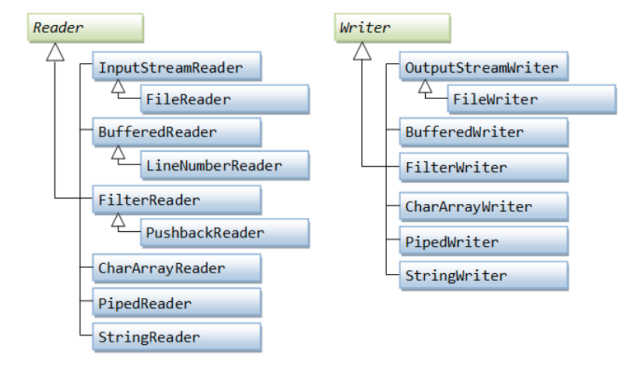
\includegraphics[scale=0.6]{imagenes/rw.png}
%\end{figure}
%\end{frame}

%\begin{frame}[fragile]
%\frametitle{FileWriter \& FileReader}
%Copiando un fichero de texto:
%\begin{footnotesize}
%\begin{verbatim}
%import java.io.File;
%import java.io.FileReader;
%import java.io.FileWriter;
%import java.io.IOException;

%public class Copia {
%  public static void main(String[] args)
%   throws IOException {
%    File inputFile = new File("in.txt");
%    File outputFile = new File("out.txt");
%    FileReader in = new FileReader(inputFile);
%    FileWriter out = new FileWriter(outputFile);
%    int c;

%    while ((c = in.read()) != -1)
%      out.write(c);

%    in.close();
%    out.close();
%  }
%}
%\end{verbatim}
%\end{footnotesize}
%\end{frame}

%\begin{frame}[fragile]
%\frametitle{BufferedReader \& BufferedWriter}
%\begin{itemize}[<+->]
%\item Se usan para envolver FileWriter y FileReader
%\item Mejora el rendimiento de ambos.
%\item Pues usamos un buffer de memoria.
%\item Además provee un nuevo método \emph{readLine()}
%\end{itemize}
%\end{frame}

%\begin{frame}[fragile]
%\frametitle{Ejemplo BufferedReader \& BufferedWriter}
%\begin{tiny}
%\begin{verbatim}
%import java.io.*;
%// Write a text message to an output file, then read it back.
%// FileReader/FileWriter uses the default charset for file encoding.
%public class BufferedFileReaderWriterJDK7 {
%   public static void main(String[] args) {
%      String strFilename = "out.txt";
%      String message = "Hello, world!\nHello, world again!\n";  

%      // Print the default charset
%      System.out.println(java.nio.charset.Charset.defaultCharset());
 
%      try (BufferedWriter out = new BufferedWriter(new FileWriter(strFilename))) {
%         out.write(message);
%         out.flush();
%      } catch (IOException ex) {
%         ex.printStackTrace();
%      }
 
%      try (BufferedReader in = new BufferedReader(new FileReader(strFilename))) {
%         String inLine;
%         while ((inLine = in.readLine()) != null) {  // exclude newline
%            System.out.println(inLine);
%         }
%      } catch (IOException ex) {
%         ex.printStackTrace();
%      }
%   }
%}
%\end{verbatim}
%\end{tiny}
%\end{frame}





\section{I/O Formateado}
\begin{frame}[fragile]
\frametitle{Clase Scanner}
\begin{itemize}[<+->]
\item JDK 1.5 introduce java.util.Scanner.
\item Parsea tokens usando diferentes métodos \emph{nextInt(), nextByte(), nextShort(), nextLong(), nextFloat(), nextDouble(), nextBoolean(), next() for String, y nextLine()}
\item Existen métodos \emph{hasNextXxx()} para chequear la disponibilidad de la entrada.
\end{itemize}
\end{frame}


\begin{frame}[fragile]
\frametitle{Clase Scanner}
\begin{tiny}

\begin{block}{Constructores}
\begin{verbatim}
public Scanner(File source) throws FileNotFoundException
public Scanner(File source, String charsetName) throws FileNotFoundException
// Para System.in
public Scanner(InputStream source)
public Scanner(InputStream source, String charsetName)
// para un String
public Scanner(String source)
\end{verbatim}
\end{block}
\pause
\begin{block}{Ejemplo}
\begin{verbatim}
// Construye un Scanner para parsear un int desde teclado
Scanner in1 = new Scanner(System.in);
int i = in1.nextInt();
 
// Construye un Scanner para parsear los dobles de un fichero
Scanner in2 = new Scanner(new File("in.txt"));   FileNotFoundException
while (in2.hasNextDouble()) {
   double d = in.nextDouble();
}
 
// Construye un Scanner para parsear  string
Scanner in3 = new Scanner("This is the input text String");
while (in3.hasNext()) {
   String s = in.next();
}
\end{verbatim}
\end{block}
\end{tiny}
\end{frame}

\begin{frame}[fragile]
\frametitle{Scanner y el método useDelimiter()}
\begin{itemize}[<+->]
\item \emph{useDelimiter (pattern)}
\item Establece el delimitador para crear \emph{tokens}
\item Ejemplo:
\end{itemize}
\pause
\begin{footnotesize}
\begin{verbatim}
import java.util.Scanner;

public class ScannerTokenizingText {
   public static void main(String[] args) {
      String text = "4231, Java Programming, 1000.00";
      Scanner scanner = new Scanner(text).useDelimiter("\\s*,\\s*");
      int checkNumber = scanner.nextInt();
      String description = scanner.next();
      float amount  = scanner.nextFloat();
      System.out.printf("/***** Tokenizing Text *****/\n\n");
      System.out.printf("String to tokenize: %s\n", text);
      System.out.printf("checkNumber: %d\n", checkNumber);
      System.out.printf("description: %s\n", description);
      System.out.printf("amount: %f", amount);
   }
}
\end{verbatim}
\end{footnotesize}
\end{frame}

\begin{frame}[fragile]
\frametitle{String.format}
\begin{itemize}[<+->]
\item Su compartamiento es similar al de \emph{printf}
\item Se usa un \emph{patrón de formateo}
\item Los parámetros separados por comas.
\item Ejemplos:
\end{itemize}
\pause
\begin{footnotesize}
\begin{verbatim}
int edad = 28;
String nombre = "David";
String patron = "El nombre de la persona es %s y tiene %d años";
String resultado = String.format(patron,nombre,edad);
System.out.print(resultado)  
//El nombre de la persona es David y tiene 28 años
\end{verbatim}
\pause
\begin{verbatim}
int hora = 13;
int minutos = 45;
String nombre = "David";
String patron = "%s ha accedido a las %d:%d h";
String resultado = String.format(patron,nombre,hora,minutos);
System.out.print(resultado);
// David ha accedido a las 13:45 h
\end{verbatim}
\end{footnotesize}
\end{frame}

\section{File I/O in JDK 1.7}
\subsection{Interface java.nio.file.Path}
\begin{frame}[fragile]
\frametitle{Helper class java.nio.file.Paths}
\begin{verbatim}
public static Path get(String first, String... more)
// Este método acepta varios argumentos).
// Los une formanod un objeto Path.
// La locat¡lizació del Path puede o no existir.  
  
public static Path get(URI uri)
// Convierte el URI a un objeto Path.
\end{verbatim}
Ejemplos:
\begin{verbatim}
Path p1 = Paths.get("in.txt");     
Path p2 = Paths.get("c:\\myproejct\\java\\Hello.java");  
Path p3 = Paths.get("/use/local");  
\end{verbatim}
\end{frame}

\begin{frame}[fragile]
\frametitle{Ejemplo}
\begin{tiny}
\begin{verbatim}
import java.nio.file.*;
public class PathInfo {
   public static void main(String[] args) {
      // Windows
      Path path = Paths.get("D:\\myproject\\java\\test\\Hello.java");
      // Unix/Mac
      //Path path = Paths.get("/myproject/java/test/Hello.java");
 
      // Print Path Info
      System.out.println("toString:    " + path.toString());    // D:\myproject\java\test\Hello.java
      System.out.println("getFileName: " + path.getFileName()); // Hello.java
      System.out.println("getParent: " + path.getParent());     // D:\myproject\java\test
      System.out.println("getRoot: " + path.getRoot());         // D:\
 
      // root, level-0, level-1, ...
      int nameCount = path.getNameCount();
      System.out.println("getNameCount: " + nameCount);   // 4
      for (int i = 0; i < nameCount; ++i) {
         System.out.println("getName(" + i + "): " + path.getName(i)); // (0)myproject, (1)java,
      }                                                                // (2) test, (3) Hello.java
      System.out.println("subpath(0,2): " + path.subpath(0,2));  // myproject\java
      System.out.println("subpath(1,4): " + path.subpath(1,4));  // java\test\Hello.java
   }
}
\end{verbatim}
\end{tiny}
\end{frame}

\begin{frame}[fragile]
\frametitle{Helper Class java.nio.file.Files}
\begin{tiny}
\begin{verbatim}
public static long size(Path path)  // Returns the size of the file
 
public static boolean exists(Path path, LinkOption... options)
// Verificas si el Path existse como un file/directory/symlink.
// si devuelve false si el file no existe
// LinkOption especifica como symlink deberían se meneados, 
//   ejmplo: NOFOLLOW_LINKS: no seguir enlaces.
public static boolean notExists(Path path, LinkOption... options)     // ¿Existe?
 
public static boolean isDirectory(Path path, LinkOption... options)   // ¿Directorio?
public static boolean isRegularFile(Path path, LinkOption... options) // ¿Fichero?
public static boolean isSymbolicLink(Path path)                       // ¿Enlace?
 
public static boolean isReadable(Path path)    // ¿permiso lectura?
public static boolean isWritable(Path path)    // ¿permiso escritura?
public static boolean isExecutable(Path path)  // ¿permiso ejecuión?
\end{verbatim}
\end{tiny}
\end{frame}

\begin{frame}[fragile]
\frametitle{Otros métodos}
\begin{verbatim}
public static void delete(Path path) throws IOException
public static boolean deleteIfExists(Path path)
   throws IOException
\end{verbatim}
\pause
\begin{verbatim}
public static Path copy(Path source, Path target, 
   CopyOption... options) throws IOException
public static Path move(Path source, Path target, 
   CopyOption... options) throws IOException
\end{verbatim}
CopyOption: REPLACE\_EXISTING, COPY\_ATTRIBUTES, NOFOLLOW\_LINKS
\pause
\end{frame}

\begin{frame}[fragile]
\frametitle{Otros métodos}
\begin{scriptsize}

\begin{verbatim}
public static byte[] readAllBytes(Path path) throws IOException
// Lee todos los bytes y devuelve byte[]. 
public static Path write(Path path, byte[] bytes,
   OpenOption... options) throws IOException
// Opciones spn: CREATE, TRUNCATE_EXISTING, y WRITE
\end{verbatim}
\pause
\begin{verbatim}
public static List<String> readAllLines(Path path, Charset cs)
    throws IOException
// Lee todas las líneas.
// Terminador de línea puede ser "\n", "\r\n" or "\r".
public static Path write(Path path, Iterable<? extends CharSequence> lines, 
   Charset cs, OpenOption... options) throws IOException
\end{verbatim}

\end{scriptsize}%\pause
\end{frame} 	

\begin{frame}[fragile]
\frametitle{Crear ficheros, directorios o enlaces}
\begin{footnotesize}
\begin{verbatim}
ppublic static Path createFile(Path path, FileAttribute<?>... attrs)
// Crea un nuevo fichero.

public static Path createDirectories(Path dir, FileAttribute<?>
   ... attrs) throws IOException
// Crea un nuevo directorio.

public public static Path createSymbolicLink(Path link, Path target,
   FileAttribute<?>... attrs) throws IOException
// Creates un enlace simbólico
\end{verbatim}
\end{footnotesize}
\end{frame}

\begin{frame}
\frametitle{FIN}
\begin{figure}

\includegraphics[scale=0.35]{imagenes/fing.jpg}
\end{figure}
\end{frame}

\end{document}